\documentclass{beamer}
\usepackage[latin1]{inputenc}
%\usetheme{Montpellier}
%\usetheme{Boadilla}
%\usecolortheme[RGB={204,51,255}]{structure}
%\usecolortheme[named=purple]{structure}
\usecolortheme[RGB={128,62,62}]{structure}
%\definecolor{dark}{rgb}{0.3,0.15,0.3}
%\definecolor{light}{rgb}{0.8,0.6,0.8}
%\definecolor{reddish}{rgb}{.5,0.15,0.15}
\definecolor{dark}{rgb}{0.5,0.3,0.4}
%\definecolor{light}{rgb}{0.8,0.6,0.8}
\definecolor{reddish}{rgb}{.7,0.25,0.25}
\definecolor{greenish}{rgb}{.25,0.7,0.25}
\definecolor{blueish}{rgb}{.25,0.25,0.7}
\definecolor{purple}{rgb}{.5,0.0,0.5}
\usepackage{graphicx}
\usepackage{pstricks}

\usepackage{amssymb}

\usepackage{amsmath}
\setbeamertemplate{navigation symbols}{}

\newcommand{\crish}{\color{reddish}}
\newcommand{\cbla}{\color{black}}
\newcommand{\cred}{\color{red}}
\newcommand{\cblu}{\color{blue}}

\newcommand{\sm}{\color{reddish}$}
\newcommand{\fm}{$\color{black}}
\usepackage{tikz}
\usetikzlibrary{arrows,decorations.markings,positioning}
\usepackage{epstopdf}
\title{Lecture 1: Introducing probability}
\author{COMS10014 Mathematics for Computer Science A}
\institute{\texttt{cs-uob.github.io/COMS10014/ and github.com/coms10011/2021\_22}}
\date{November 2021}
\begin{document}
\maketitle
\begin{frame}{What is probability?}
  \begin{quote}
    Probability is a set of mathematical definitions and theorems that
    are useful for reasoning about randomness and uncertainty
  \end{quote}
\end{frame}

\begin{frame}{Working out probabilities}
  \begin{center}
    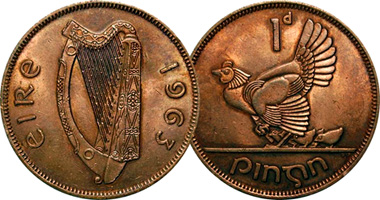
\includegraphics[width=3cm]{1d.jpg}
    \end{center}
  A fair coin has a one in two chance of turning up heads, if each spin is independent it has a probability of
  \crish$$P(\mbox{six heads in a row})=\left(\frac{1}{2}\right)^6=0.015625$$\cbla{}
\end{frame}

\begin{frame}{Frequentist statistics}
    \begin{center}
    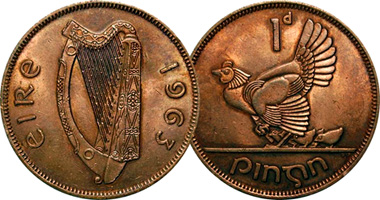
\includegraphics[width=3cm]{1d.jpg}
    \end{center}
A fair coin has a 1.5\% chance of coming up heads six times in a row,
so if you spun a coin six times and it came up heads each time you can
be 98.5\% certain the coin is not fair, maybe.
\end{frame}

\begin{frame}{Frequentist statistics}
    \begin{center}
    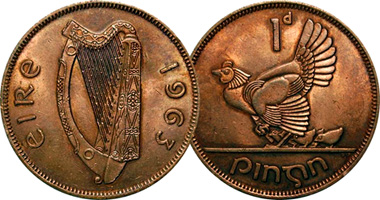
\includegraphics[width=3cm]{1d.jpg}
    \end{center}
A fair coin has a 1.5\% chance of coming up heads six times in a row,
so if you spun a coin six times and it came up harps each time you can
be 98.5\% certain the coin is not fair, maybe.
\cblu{}
If you include all heads and heads-harps-heads-harps-heads-harps and
harps-heads-harps-heads-harps-heads in your list of `weird' outcomes
then there is a 6$\%$ chance of getting a `weird' outcome.\cbla{}
\end{frame}

\begin{frame}{Bayesian statistics}
  \cred{}Aoife\cbla{}  tells \cblu{}Brendan\cbla{}  she has spun a coin six times and taken down the
  sequence. As far as \cblu{}Brendan\cbla{}  is concerned all 64 outcomes are equally
  likely. Now, \cred{}Aoife\cbla{}  tells \cblu{}Brendan\cbla{}  the coin turned out the same each
  time, so \cblu{}Brendan\cbla{}  updates his belief about the sequence; he now
  believes there are two possibilities, all heads and all harps, each
  equally likely.
\end{frame}


\begin{frame}{What is probability?}
  \begin{quote}
    Probability is a set of mathematical definitions and theorems that
    are useful for reasoning about randomness and uncertainty
  \end{quote}
\end{frame}

\begin{frame}{Some definitions - sample space}
  A \textbf{sample space} is a set of possible outcomes. 
\end{frame}

\begin{frame}{Sample space}
  To model the experiment where a coin is tossed once we'd use
  \crish$$S=\{H,T\}$$\cbla{}
  where \crish$H$\cbla{} and \crish$T$\cbla{} correspond to heads and harps.
\end{frame}


\begin{frame}{Sample space}
  To model the experiment where a coin is tossed twice in a row we'd use
  \crish$$S=\{HH,HT,TH,TT\}$$\cbla{}
  and where two coins are tossed and we don't distinguish one from the other
  \crish$$S=\{HH,HT,TT\}$$\cbla{}
  where \crish$HT$\cbla{} stands for heads and harps in any order.
\end{frame}

\begin{frame}{Infinite sample spaces}
  If you wanted to model the number of coin tosses before you get a head you'd use
  \crish$$S=\mathbb{N}$$\cbla{}
  and to model the height of trees
  \crish$$S=[0,\infty)$$\cbla{}
\end{frame}

\begin{frame}{Some definitions - event}

  An \textbf{event} in a sample space \crish$X$\cbla{} is a subset \crish$E\subset X$\cbla{}.

\end{frame}

\begin{frame}{Event}
\begin{center}
    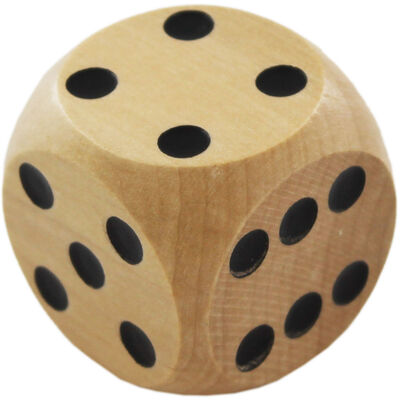
\includegraphics[width=2cm]{dice.jpg}
\end{center}  
If we have sample space \crish$$S=\{1,2,3,4,5,6\}$$\cbla{} corresponding to the
face values of a dice\footnote{or die - originally \textsl{dice} was the plural of \textsl{die}}, then the set of even sides \crish$$E=\{2,4,6\}$$\cbla{} is an
example event. This might be useful for working out the probability of an even roll.
\end{frame}

\begin{frame}{Some definitions - probability}
Formally, a \textbf{probability} is a map \crish$P$\cbla{}  from
events to real numbers such that:
\begin{enumerate}
\item \crish$P(A)\ge 0$\cbla{}  for all events.
\item \crish$P(X)=1$\cbla{} 
\item If \crish$A\cap B=\emptyset$\cbla{}  for two events \crish$A$\cbla{}  and \crish$B$\cbla{}  then 
\crish$$
P(A\cup B)=P(A)+P(B)
$$\cbla{}
\end{enumerate}
\end{frame}  

\begin{frame}{Some definitions - probability mass function}
The \textbf{probability mass function} is a map \crish$p$\cbla{}  from outcomes to real numbers such that:
\begin{enumerate}
\item \crish$p(x)\ge 0$\cbla{}  for all \crish$x\in X$\cbla{} 
\item \crish$\sum_{x\in X} p(x)=1$\cbla{} 
\end{enumerate}
\end{frame}

\begin{frame}{The probability and the probability mass function}
\crish$$
P(A)=\sum_{x\in A}p(x)
$$\cbla{}
\end{frame}

  
\end{document}
